%\documentclass[letterpaper, onecolumn, 10pt]{article}
%\linespread{2.4}
\documentclass[letterpaper, twocolumn, 10pt]{article}
\usepackage{usenix2019,endnotes}
%\linespread{0.99}

\usepackage{multirow}
\usepackage{comment}
\usepackage{epsfig}
\usepackage{kotex}
%\usepackage{amsmath}
\usepackage{amssymb}
\usepackage{multirow}
\usepackage{url}
\usepackage{subfig}
\usepackage{color}
\usepackage{xcolor}
\usepackage{cases}
\usepackage{graphicx}
%\usepackage{float}
\usepackage{caption}
\usepackage[draft]{pgf}
\usepackage[normalem]{ulem}


\renewcommand{\figurename}{Fig.}
\newcommand{\note}[1]{{\color{blue}{#1}}}
\newcommand{\error}[1]{{\color{red}{#1}}}

\begin{document}

\title{
\bf Fully Automatic Stream Management for Multi-Streamed SSDs \\ Using Program Contexts}

%\numberofauthors{1}

\author{
{\rm Submission \#22} \\
}



%\numberofauthors{1}
%
%\author{
%	{\rm Taejin Kim$^1$, Sangwook Shane Hahn$^1$, Sungjin Lee$^2$,} \\ 
%	{\rm Jooyoung Hwang$^3$, Jongyoul Lee$^3$, and Jihong Kim$^1$} \\
%	\and
%	$^1$Seoul National University, $^2$DGIST, $^3$Samsung Electronics
%	}


\maketitle
%\thispagestyle{empty}
%\pagestyle{empty}
\subsection*{Abstract}
\vspace{-6pt}
Multi-streamed SSDs can significantly improve both the performance and lifetime
of flash-based SSDs when their streams are properly managed.  However, existing
stream management solutions do not adequately support the multi-streamed SSDs
for their wide adoption.  No existing stream management technique works in a
fully automatic fashion for general I/O workloads including append-only
workloads.  Furthermore, the limited number of available streams makes it
difficult to effectively manage streams when a large number of streams are
required.  In this paper, we propose a {\it fully automatic} stream management
technique, \textsf{\small PCStream}, which can work efficiently for {\it
general} I/O workloads.  \textsf{\small PCStream} is based on the key insight
that stream allocation decisions should be made on dominant I/O activities. By
identifying dominant I/O activities using program contexts, \textsf{\small
PCStream} fully automates the whole process of stream allocation within the
kernel with no manual work.  In order to overcome the limited number of
supported streams, we propose a new type of streams, internal streams, which
can be implemented at low cost.  \textsf{\small PCStream} can effectively
double the number of available streams using internal streams.  Our evaluations
on real multi-streamed SSDs show that \textsf{\small PCStream} achieves the
same efficiency as highly-optimized manual allocations by experienced
programmers.  \textsf{\small PCStream} improves IOPS by up to \error{56\%} over the
existing automatic technique by reducing the garbage collection overhead by up
to \error{69\%}.

\vspace{-12pt}
\section{Introduction}
\label{sec:intro}
\vspace{-4pt}
In flash-based SSDs, garbage collection (GC) is inevitable because NAND flash
memory does not support in-place updates.  Since the efficiency of garbage
collection significantly affects  both the performance and lifetime of SSDs,
garbage collection has been extensively investigated so that the garbage
collection overhead can be reduced ~\cite{DAC, WriteAmplification, GCGreedy,
GCVictim, GCTTFlash, HotCold}.  For example, hot-cold separation techniques are
commonly used inside an SSD so that quickly invalidated pages are not mixed
with long-lived data in the same block.   For more efficient garbage
collection, many techniques also exploit host-level I/O access characteristics
which can be used as useful hints on the efficient data separation inside the
SSD~\cite{JiTGC, ShadowGC}.

Multi-streamed SSDs provide a special interface mechanism for a host system,
called streams\endnote{In this paper, we use ``streams'' and ``external
streams'' interchangeably.}, which data separation decisions {\it on the
host level} can be delivered to SSDs~\cite{T10, MultiStream}.  When the host
system assigns two data $D_1$ and $D_2$ to different streams $S_1$ and $S_2$,
respectively, a multi-streamed SSD places $D_1$ and $D_2$ in different blocks,
which belong to $S_1$ and $S_2$, respectively.  When $D_1$ and $D_2$ have
distinct update patterns, say, $D_1$ with a short lifetime and $D_2$ with a
long lifetime, allocating $D_1$ and $D_2$ to different streams can be helpful
in minimizing the copy cost of garbage collection by separating hot data from
cold data.  Since data separation decisions can be made more intelligently on
the host level over on the SSD level, when streams are properly managed, they
can significantly improve both the performance and lifetime of flash-based
SSDs~\cite{MultiStream, Level,vStream, FStream, AutoStream}.  We assume that a
multi-streamed SSD supports $m$+1 streams, $S_0$, ..., $S_{m}$.

In order to maximize the potential benefit of multi-streamed SSDs in practice,
several requirements need to be satisfied both for stream management and for
SSD stream implementation.  First, stream management should be supported in a
fully automatic fashion over general I/O workloads without any manual work.
For example, if an application developer should manage stream allocations {\it
manually} for a given SSD, multi-streamed SSDs are difficult to be widely
employed in practice.   Second, stream management techniques should have no
dependency on the number of available streams.  If stream allocation decisions
have some dependence on the number of available streams,  stream allocation
should be modified whenever the number of streams in an SSD changes.  Third,
the number of streams supported in an SSD should be sufficient to work well
with multiple concurrent I/O workloads.  For example, with 4 streams, it would
be difficult to support a large number of I/O-intensive concurrent tasks.  

Unfortunately, to the best of our knowledge, no existing solutions  for
multi-streamed SSDs meet all these requirements.  Most existing
techniques~\cite{MultiStream, Level, vStream, FStream} require programmers to
assign streams at the application level with manual code modifications.
\textsf{\small AutoStream}~\cite{AutoStream} is the only known automatic
technique that supports stream management in the kernel level without manual
stream allocation.  However, since \textsf{\small AutoStream} predicts data
lifetimes using the update frequency of the logical block address (LBA), it
does not work well with append-only workloads (such as
RocksDB~\cite{RocksDB} or Cassandra~\cite{Cassandra})
and write-once workloads (such as a Linux kernel build).  Unlike conventional
in-place update workloads where data written to the same LBAs often show strong update
locality, append-only or write-once workloads make it impossible to predict data lifetimes
from LBA characteristics such as the access frequency.

In this paper, we propose a {\it fully-automatic} stream management technique,
called \textsf{\small PCStream}, which works efficiently over general I/O
workloads including append-only, write-once as well as in-place update workloads.   
The key insight behind
\textsf{\small PCStream} is that stream allocation decisions should be made at
a higher abstraction level where {\it I/O activities}, not LBAs, can be
meaningfully distinguished.  For example, in RocksDB, if we can tell whether
the current I/O is a part of a logging activity or a compaction activity, stream
allocation decisions can be made a lot more efficiently over when only LBAs of
the current I/O is available.   

In \textsf{\small PCStream}, we employ a write program context\endnote{
Since we are interested in write-related system calls such as write() in
Linux, we use {\it write program contexts} and {\it program contexts}
interchangeable where no confusion arises.} as such a higher-level
classification unit for representing I/O activity regardless of the type of I/O
workloads.  A program context (PC)~\cite{PC, PC2}, which uniquely represents an
execution path of a program up to a write system call, is known to be effective
in representing dominant I/O activities~\cite{PCHa}.  Furthermore, most
dominant I/O activities tend to show distinct data lifetime characteristics.
By identifying dominant I/O activities using program contexts during run time,
\textsf{\small PCStream} can automate the whole process of stream allocation
within the kernel with no manual work.  In order to seamlessly support various
SSDs with different numbers of streams, \textsf{\small PCStream} groups program
contexts with similar data lifetimes depending on the number of supported
streams using the k-means clustering algorithm~\cite{kmeans}.  Since program
contexts focus on the semantic aspect of I/O execution as a lifetime
classifier, not on the low-level details such as LBAs and access patterns,
\textsf{\small PCStream} easily supports different I/O workloads regardless of
whether it is update-only or append-only.   

Although many program contexts show that their data lifetimes are narrowly
distributed, we observed that this is not necessarily true because of several
reasons.  For example, when a single program context handles multiple types of
data with different lifetimes, data lifetime distributions of such program
contexts  have rather large variances.  In \textsf{\small PCStream}, when such
a program context {\it $PC_j$} is observed (which was mapped to a stream {\it
$S_k$}), the long-lived data of {\it $PC_j$} are moved to a different stream
{\it $S_{k'}$} during GC.  The stream {\it $S_{k'}$} prevents the long-lived
data of the stream {\it $S_k$} from being mixed with future short-lived data of
the stream {\it $S_k$}.

When several program contexts have a large variance in their data lifetimes,
the required number of total streams can quickly increase to distinguish data
with different lifetimes.
%if streams can efficiently distinguish data with different lifetimes.
In order to effectively increase the number of streams, we propose a new stream
type, called an internal stream, which can be used only for garbage collection.
Unlike external streams, internal streams can be efficiently implemented at low
cost without increasing the SSD resource budget.  In the current version of
\textsf{\small PCStream}, we create the same number of internal streams as the
external streams, effectively doubling the number of available streams. 

In order to evaluate the effectiveness of \textsf{\small PCStream}, we have
implemented \textsf{\small PCStream} in the Linux kernel (ver. 4.5) and
extended a Samsung PM963 SSD to support internal streams.  Our experimental
results show that \textsf{\small PCStream} can reduce the GC overhead as much
as a manual stream management technique while requiring no code modification.
Over \textsf{\small AutoStream}, \textsf{\small PCStream} improves the average
IOPS by 28\% while reducing the average WAF by 49\%.

The rest of this paper is organized as follows.  
%In Section 2, we explain the key limitations of existing stream management techniques and stream implementation methods.  
In Section 2, we review existing stream management techniques.
Before describing \textsf{\small PCStream}, its two
core components are presented in Sections 3 and 4.  Section 5 describes
\textsf{\small PCStream} in detail.  Experimental results follow in Section 6,
and related work is summarized in Section 7.  Finally, we conclude with a
summary and future work in Section 8.


\section{Limitations of Current Practice in Multi-Streamed SSDs}
In this section, we review the key weaknesses of existing stream management techniques 
as well as stream implementation methods.  
PCStream was motivated to overcome these weaknesses so that multi-streamed
SSDs can be widely employed in practice.

\subsection{No Automatic Stream Management for General I/O Workloads}
Most existing stream management techniques~\cite{MultiStream, Level, vStream} 
require programmers to manually allocate streams for their applications.

{\color{blue}
For example, 
in both ManualStream and vStream, there is no systematic guildeline on how to
allocate streams for a given application. 
The efficiency of stream allocations largely depends on the programmer's 
understanding and expertise on data temperature (i.e., frequency of updates)
and internals of file systems/database systems.
}
Furthermore, these
techniques also assume that the number of streams is known {\it a priori}.  
Therefore, when an SSD with a different number of streams is used, 
these techniques need to re-allocate streams manually.
A recently proposed \textsf{\small vStream}~\cite{vStream} 
technique is an exception to this 
restriction by allocating streams to virtual streams, not physical streams.  
However, even in \textsf{\small vStream}, virtual stream allocation is left to
programmer's decisions.

{\color{blue}
Although \textsf{\small FStream} and \textsf{\small AutoStream} may be considered 
as automatic stream management techniques,
their applicability is quite limited.
\textsf{\small FStream} can be useful for separating file system metadata but it does not
work for the user data separation.
\textsf{\small AutoStream}~\cite{AutoStream} is the only known technique that works in a 
fully automatic fashion by making stream allocation decisions within 
the kernel.
However, since \textsf{\small AutoStream} predicts data lifetimes using the
access frequency of the same LBA, \textsf{\small AutoStream} does not work
well with recent data-intensive 
applications where a majority of
new data are written in an append-only manner.  
}

In order to illustrate a mismatch between an LBA-based predictor and 
append-only workloads, we analyzed the write pattern of 
RocksDB~\cite{RocksDB}, which is a
popular key-value store based on the LSM-tree algorithm~\cite{LSM}.
Fig.~\ref{fig:lba_lifetime}(a) shows how LBAs may be related 
to data lifetimes in RocksDB~\cite{RocksDB}.  
{\color{blue}
We define the lifetime of data as the interval length (in terms of
the logical time based on the number of writes) between
the data is first written and when the data is invalidated
by an overwrite or a TRIM command.
}
As shown in Fig.~\ref{fig:lba_lifetime}(a), 
there is no strong correlation between LBAs and lifetimes in RocksDB.  
This scatter plot is in sharp contrast with one for update workloads 
where a few distinct LBA regions have short lifetimes while others 
have very long lifetimes.

\begin{figure}[t]
	\centering
	\hfill
	%\vspace{-9pt}
	%\captionsetup[subfigure]{margin={0cm,1cm}}
	\subfloat[Lifetime patterns over LBAs]{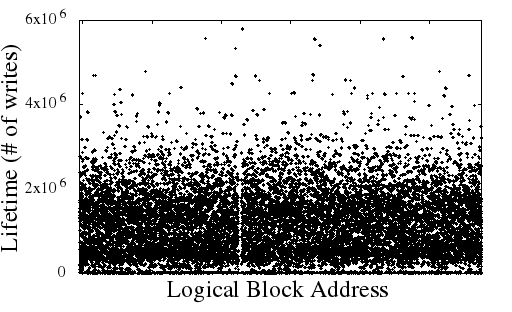
\includegraphics[width=0.215\textwidth]{figure/lba_lifetime2}}  % data from 0/03031641
	\hspace{10pt}
	\subfloat[Lifetime patterns over time]{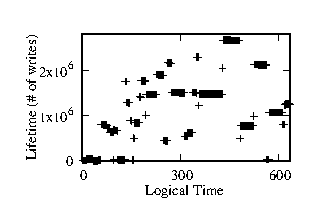
\includegraphics[width=0.21\textwidth]{figure/lifetime_in_chunk}}
	%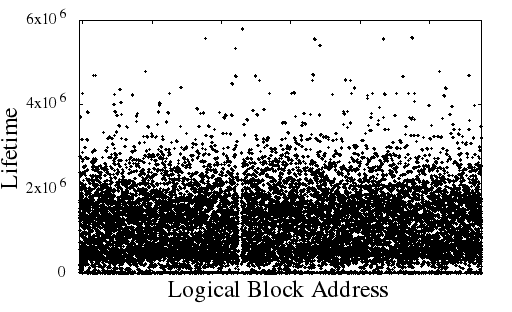
\includegraphics[width=0.9\linewidth]{figure/lba_lifetime} 
	%\vspace{-3pt}
	\caption{Lifetime distributions of append-only workload over addresses and times.} %shane part
	\label{fig:lba_lifetime}
	%\vspace{-20pt}
\end{figure}


We also analyzed 
if the lifetimes of LBAs change under some predictable patterns over time 
although the overall lifetime distribution shows large variances.
Fig.~\ref{fig:lba_lifetime}(b) shows a scatter plot of data lifetimes over the logical time 
for a specific 1-MB chunk with 256 pages. 
As shown in Fig.~\ref{fig:lba_lifetime}(b), 
for the given chunk, data lifetimes vary in a random fashion
(although some temporal locality is observed).
Over the logical time, the lifetime of data written to the chunk 
varies in an unpredictable fashion.  
For example, at the logical time 10, the lifetime was 1 but it increases about 
2.6 million around the logical time 450 
followed by a rapid drop around the logical time 600. 
Our illustration using RocksDB strongly suggests that under append-only workloads, 
{\color{blue}LBAs are not meaningful in predicting data lifetimes reliably.
In order to support {\it general} I/O workloads in an automatic fashion, stream 
management decisions should be based on higher-level information
which do not depend on lower-level details such as write patterns of successive LBAs.
}

\subsection{Limited Number of Supported Streams}
One of the key performance parameters in multi-streamed SSDs is the number of 
available streams in SSDs.  
Since the main function of  streams is to separate data with different lifetimes 
so that they are not mixed in the same block, it is clear that the 
higher the number of streams, the more efficient the performance of multi-streamed SSDs.
For example, the SSD performance keeps improving as the number of streams increases 
until data with different lifetimes are allocated to separate streams.   
In order to support a large number of streams, the SBC-4 and NVMe revision 1.3, which define the 
multi-stream related specifications, allow up to 65,536 streams~\cite{T10, NVMe}.  
However, the number of streams supported in
commercial SSDs is quite limited, say, 4 to 16~\cite{MultiStream, Level, AutoStream}, 
{\color{blue}
because of several implementation constraints such as backup power capacity and the memory size.
In the SSD, a write buffering mechanism is commonly used to manage the size difference 
between the FTL mapping unit and the flash program unit and to efficiently utilize 
the high-degree of SSD internal parallelism for high performance. 
And the buffering mechanism requires a backup power resource and a fast memory resource.

In data centers or storage servers where multi-streamed SSDs are used,
in order to guarantee the data integrity even under sudden power-off conditions, 
SSDs use tantalum or electrolytic capacitors as a backup power source.  
When a main power is suddenly failed, the backup power is used to write back the
buffered data reliably.  
Since the capacity of backup power is limited because of the limited PCB size and 
its cost, the maximum amount of buffered data is also limited.  
In multi-streamed SSDs where
each stream needs its own buffered area, the amount of buffered data increases 
as the number of streams increases.  
The practical limit in the capacity of backup power, therefore, dictates the maximum
number of streams as well.

The limited size of fast memory, such as TCM or SRAM, is another main hurdle in increasing 
the number of streams in multi-streamed SSDs.
Since multi-stream related metadata which includes data structes for write buffering 
should be accessed quickly as well as frequently, 
most SSD controllers implement multi-stream data structures on fast memory than more common DRAM. 
Since the buffered write data is the latest data, 
it is always necessary to check whether there is requested LBA 
among the buffered data at the time of read request processing.
To effectively implement this check process, a hash table or bloom filter can be used, 
and buffered LBA information and buffer address are managed.
Placing these data structures in slower memory is not desirable 
because the read processing speed is greatly reduced.  
Furthermore, these data structures are also referred to store buffered data in NAND flash, 
the data structures must be located in fast memory for high write throughput. 
However, most SSD manufacturers are quite sensitive in increasing the size of 
fast memory because it may increase the overall SSD cost.   
A limited size of fast memory, unfortunately, restricts the number of
supported streams quite severely.
}


\section{Automatic I/O Activity Management Using Program Contexts}
\label{sec:programcontext}
%In developing \textsf{\small PCStream}, our key insight was that in most
%applications, (regardless of their I/O workload characteristics) a few dominant
%I/O activities exist and each dominant I/O activity   represents the
%application's important I/O context (e.g., for logging or for flushing).
%Furthermore, most dominant I/O activities tend to have distinct data lifetime
%patterns.  In order to distinguish data by their lifetimes, therefore, it is
%important to effectively distinguish dominant I/O activities from each other.
%For example, in update workloads, LBAs alone were effective in separating
%dominant I/O activities.  
\begin{figure}[t]
%	\vspace{-10pt}
	\centering
	%\vspace{-8pt}
	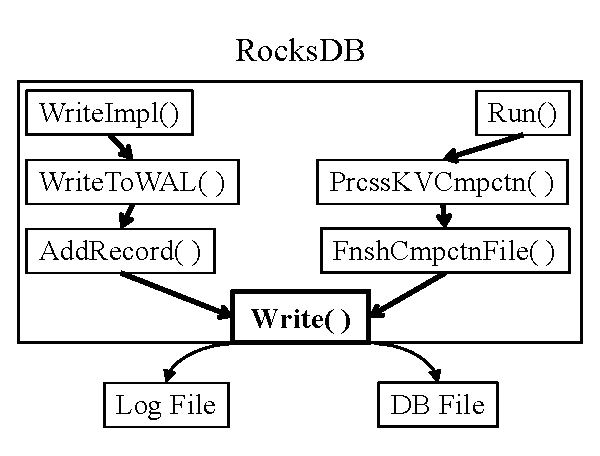
\includegraphics[width=0.3\textwidth]{figure/writepath}
	\caption{An illustration of (simplified) execution paths of two dominant I/O activities in RocksDB.}
	\label{fig:iopath}
\end{figure}

In developing an efficient data lifetime separator for general I/O workloads,
our key insight was that in most applications,
the overall I/O behavior of 
applications is decided by a few dominant
I/O activities (e.g., logging and flushing in RocksDB). 
Moreover, 
data written by dominant I/O activities tend to have distinct lifetime patterns.
Therefore, if such dominant I/O activities of applications can be 
automatically detected and distinguished each other in an LBA-{\it oblivious} fashion, 
an automatic stream management technique can be developed for widely varying I/O workloads 
including append-only workloads.
%(regardless of their I/O workload characteristics) a few dominant
%I/O activities exist and each dominant I/O activity   represents the
%application's important I/O context (e.g., for logging or for flushing).
%Furthermore, most dominant I/O activities tend to have distinct data lifetime
%patterns.  In order to distinguish data by their lifetimes, therefore, it is
%important to effectively distinguish dominant I/O activities from each other.
%For example, in update workloads, LBAs alone were effective in separating
%dominant I/O activities.  

In this paper, we argue that a program context can be
used to build an efficient general-purpose 
classifier of dominant I/O activities with different data lifetimes.
Here, a PC
represents an execution path of an application which invokes write-related
system call functions such as {\tt write()} and {\tt writev()}.  
There could be various ways of extracting PCs, 
but the most common approach~\cite{PC, PC2} is to
represent each PC with its PC signature which is computed by summing 
program counter values of all the functions along the execution path which
leads to a write system call.

%we represent the PC by summing program counter values of
%all the functions along the execution path which leads to a write system call.

\begin{figure*}[!t]
\centering
%\vspace{-10pt}
	\subfloat[RocksDB: Logging]{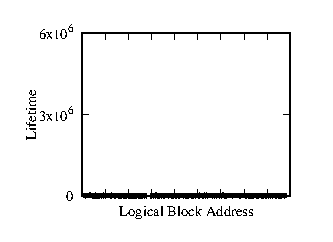
\includegraphics[width=0.22\textwidth]{figure/pcID_2}} % data from 4/03031953 
	\hspace{10pt}
	\subfloat[RocksDB: Flushing]{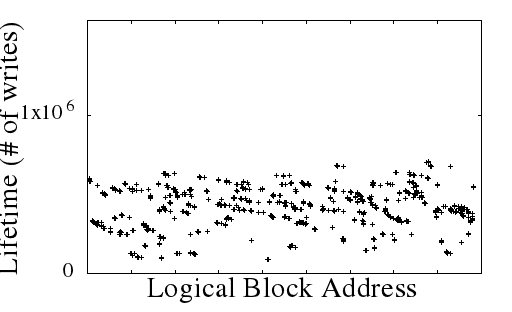
\includegraphics[width=0.22\textwidth]{figure/pcID_3}}
	\hspace{10pt}
	\subfloat[RocksDB: Compaction]{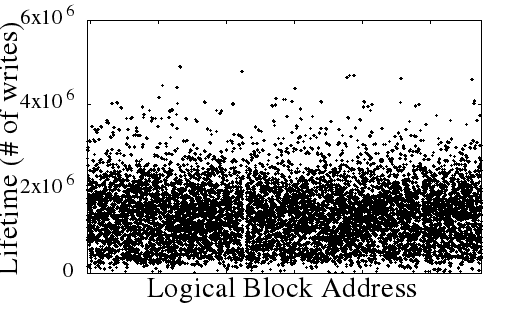
\includegraphics[width=0.22\textwidth]{figure/pc_3}}  % data from 4/03040047

	\hfill

	\subfloat[SQLite: Logging]{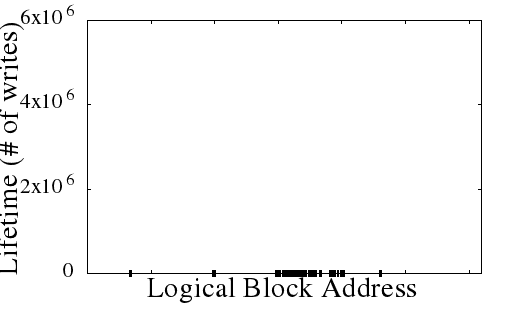
\includegraphics[width=0.22\textwidth]{figure/sqlite_short_LBA}}
	\hspace{2pt}
	\subfloat[SQLite: Updating]{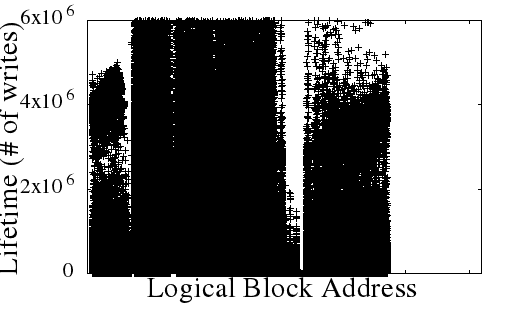
\includegraphics[width=0.22\textwidth]{figure/sqlite_long_LBA}}
	\hspace{2pt}
	\subfloat[GCC: Outputting Temp]{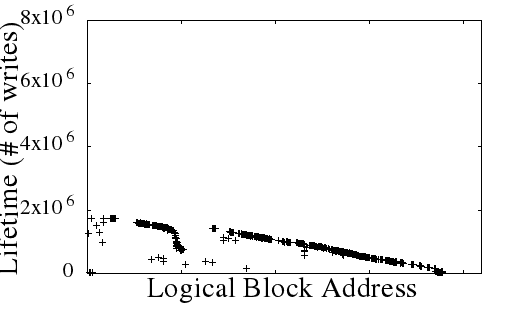
\includegraphics[width=0.22\textwidth]{figure/compile_short_PC}}
	\hspace{2pt}
	\subfloat[GCC: Outputting Executable]{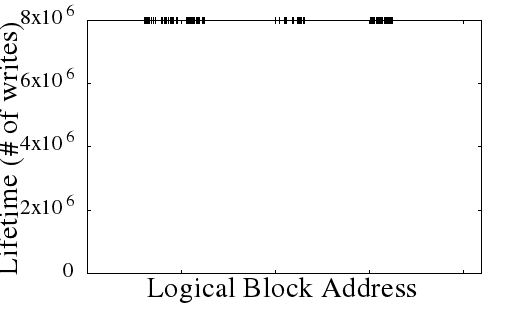
\includegraphics[width=0.22\textwidth]{figure/compile_long}}
%\vspace{-7pt}
\caption{Data lifetime distributions of dominant I/O activities in RocksDB, SQLite and GCC.} 
\label{fig:types_and_PCs}
%\vspace{-20pt}
\end{figure*}

\subsection{Program Context as a Unit of Lifetime Classification}
In order to illustrate that using PCs is an effective way to distinguish I/O
activities of an application and their data lifetime patterns, 
we measured data lifetime distributions of PCs from various applications with 
different I/O workloads.  
In this section, we report our evaluation results for three applications with distinct I/O
activities: RocksDB~\cite{RocksDB}, SQLite~\cite{SQLite}, and GCC~\cite{GCC}.
RocksDB shows the append-only workload while SQLite shows a workload 
that updates in place.
Both database workloads are expected to have distinct I/O activities 
for writing log files and data files.
GCC represents 
an extensive compiler workload (e.g., compilng a Linux kernel) that generates 
many short-lived temporary files (e.g., .s, .d, and .rc files) 
as well as some long-lived files (e.g., object files and kernel image files).

In RocksDB, dominant I/O activities include logging, flushing and compaction.
Since these I/O activities are invoked through different 
function-call paths, we can easily
identify dominant I/O activities of RocksDB using PCs.  
For example, Fig.~\ref{fig:iopath} shows 
(simplified) execution paths for 
logging and compaction in RocksDB and their PC ID values.  
The sum of program counter values of the execution path
\texttt{WriteImpl()} $\rightarrow$ \texttt{WriteToWAL()} $\rightarrow$ \texttt{AddRecord()} is used
to represent a PC for the logging activity while that of the execution path
\texttt{Run()} $\rightarrow$
\texttt{ProcessKeyValueCompaction()} $\rightarrow$ \texttt{FinishCompactionFile()} is used
for the compaction activity.

In SQLite, there exist two dominant I/O activities which are logging and managing 
database tables.
Similar to the RocksDB, SQLite writes log files and database files using different
execution paths.
In GCC, there exist many dominant I/O activities of creating various types of 
temporal files and object files.

%\textcolor{red}{(TODO: 갑자기
%lifetime 이야기가 나옴. 없애도 큰 문제가 없을 듯...) \sout{Note that using a
%program context to distinguish data lifetimes is not new. For example, Ha {\it
%et al.} proposed a data separation technique based on the program
%context~\cite{PCHa}.  However, their work was neither designed for append-only
%workloads nor for modern multi-streamed SSDs.}}

To confirm our hypothesis that data lifetimes can be distinguished by tracking
dominant I/O activities and a PC is a useful unit of classification for 
different I/O activities,
we have analyzed how well PCs work for RocksDB, SQLite and GCC.
Fig.~\ref{fig:types_and_PCs} shows data lifetime distributions of 
dominant I/O activities which were distinguished by computed PC values.
As expected, Fig.~\ref{fig:types_and_PCs} validates that dominant I/O activities 
show distinct data lifetime distributions over the logical address space.
For example, as shown in Figs.~\ref{fig:types_and_PCs}(a)$\sim$~\ref{fig:types_and_PCs}(c), 
the logging activity, the flushing activity and the compaction activity 
in RocksDB clearly exhibit quite different data lifetime distributions.
While the logged data written by the logging activity have short lifetimes, 
the flushed data by the flushing activity have little bit longer lifetimes.  
Similarly, for SQLite and GCC, dominant I/O
activities show quite distinct data lifetime characteristics as shown in 
Figs.~\ref{fig:types_and_PCs}(d)$\sim$~\ref{fig:types_and_PCs}(g).
As shown in Figs.~\ref{fig:types_and_PCs}(d), the logging activity of
SQLite generates short-lived data.  This is because SQLite overwrites logging
data in a small and fixed storage space and then removes them soon. 
Similarly,
data lifetimes of temporary files generated by GCC are 
relatively short as shown in Fig.~\ref{fig:types_and_PCs}(f),
because of the write-once pattern of temporary files.
{\color{blue}
However, unlike the other graphs in Fig.~\ref{fig:types_and_PCs}, data lifetime
distributions of Figs.~\ref{fig:types_and_PCs}(c) and ~\ref{fig:types_and_PCs}(e),
which correspond to the compaction activity of RocksDB and the updating activity of
SQLite, respectively, show large lifetime variances.
These {\it outlier I/O activities} need a special treatment, which 
will be described in Section 4.
}

Note that if we used an LBA-based data separator instead of the proposed PC-based scheme, 
most of data lifetime characteristics shown in Fig.~\ref{fig:types_and_PCs} could 
not have been known.  Only the data lifetime
distribution of the logging activity of SQLite, as shown in Fig.~\ref{fig:types_and_PCs}(d), 
can be accurately captured by the LBA-based data separator.  
For example, the LBA-based data separtor cannot 
decide that the data lifetime of data produced from the temp output activity of GCC 
is short because temporary files are not written at the same logical block addresses 
each time they are generated during
the compiling step. 


\subsection{Extracting PCs}
A PC signature, which is used as a unique ID of each program context,
is defined
to be the sum of program counters along the execution path of function calls
that finally reaches a write-related system function.  In theory, program
counter values in the execution path can be extracted in a relatively
straightforward manner.  Except for inline functions, every function call
involves pushing the address of the next instruction of a caller as a return
address to the stack, followed by pushing a frame pointer value.  By referring
to frame pointers, we are able to back-track stack frames of a process and
selectively get return addresses for generating a PC signature.
For example, Fig.~\ref{fig:getpc}(a) illustrates a stack of RocksDB corresponding
to Fig.~\ref{fig:iopath}, where return addresses are pushed before calling
the \textsf{\small  write()}, \textsf{\small AddRecord()} and \textsf{\small
WriteToWAL()} functions.  Since frame pointer values in the stack hold the
addresses of previous frame pointers, we can easily obtain return addresses and
accumulate them to compute a PC signature.  

%For example,
%Fig.~\ref{fig:getpc}(a) shows abstracted execution paths of log data and
%compaction data in RocksDB.  The return addresses are pushed before calling the
%\textsf{\small  write()}, \textsf{\small AddRecord()} and \textsf{\small
%WriteToWAL()} functions.  Fig.~\ref{fig:getpc}(b) illustrates how a PC
%signature is obtained by back-tracking the stack.  Since frame pointer values
%in the stack hold the addresses of previous frame pointers, we can easily
%obtain return addresses and accumulate them to compute a PC signature.  

The frame pointer-based approach for computing a PC signature, however, is not
always possible because modern C/C++ compilers often do not use a frame pointer
for improving the efficiency of register allocation.  One example is a {\tt
-fomit-frame-pointer} option of gcc~\cite{GCC}.  This option enables to use a frame
pointer as a general-purpose register for performance, but makes it difficult for us
to back-track return addresses along the call chains.  

\begin{figure}[t]
%	\vspace{-10pt}
	\centering
	%\vspace{-8pt}
	%\subfloat[Abstracted execution paths of two I/O activities of RocksDB.]{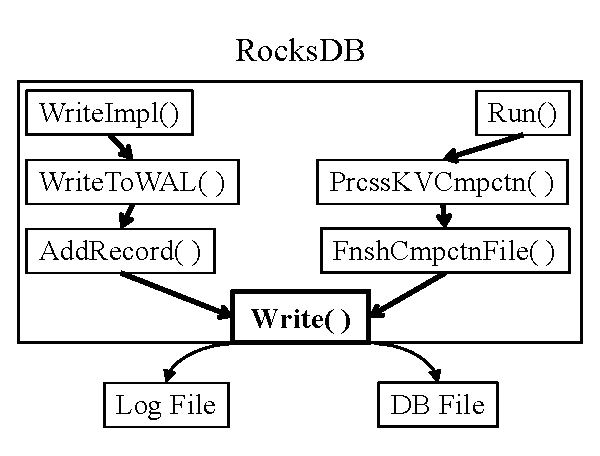
\includegraphics[width=0.3\textwidth]{figure/writepath}}  
	%\vspace{-14pt}
	%\hfill
	\subfloat[with the frame pointer.]{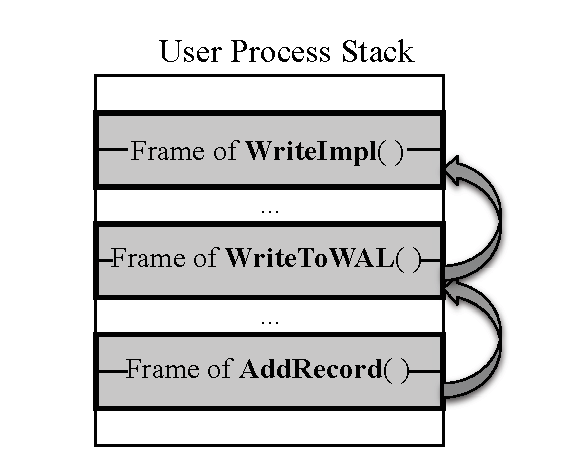
\includegraphics[width=0.22\textwidth]{figure/getpc1}}
	\hspace{4pt}
	\subfloat[without the frame pointer.]{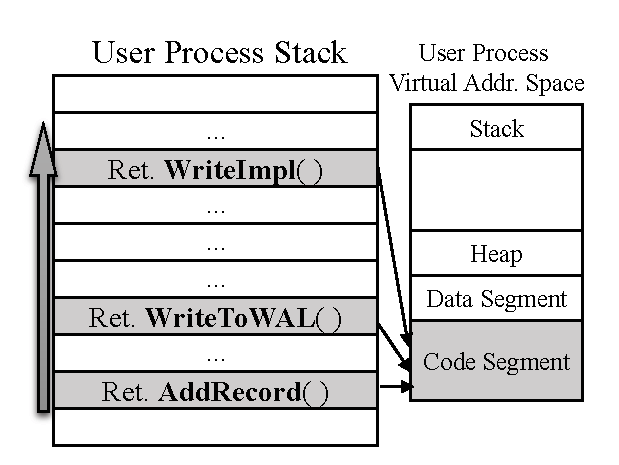
\includegraphics[width=0.22\textwidth]{figure/getpc2}}
	%\vspace{-9pt}
	\caption{Examples of PC extraction methods.}
	%\caption{An example execution path and its PC extraction.} %shane part
	\label{fig:getpc}
	%\vspace{-20pt}
\end{figure}

We employ a simple but effective workaround for back-tracking a call stack when
a frame pointer is not available.  When a write system call is made,
we scan every word in the stack
and checks if it belongs to process's code segment.  If the scanned stack word
holds a value within the address range of the code segment, it assumes that it
is a return address.  Since scanning the entire stack may takes too long, we stop
the scanning step once a sufficient number of return address candidates are found.
In the current implementation, the scanning process stops early once 
five return address candidates are identified.  
Even though it is quite ad-hoc, this restricted scan is quite effective
in distinguishing different PCs because it is very unlikely that two different PCs
reach the same write() system call through the same execution subpath 
that covers five proceeding function calls. 
In our evaluation on a PC with 3.4 GHz Intel CPU, the overhead of the
restricted scan was almost negligible, taking only 300$\sim$400 $n$sec per
\textsf{\small write()} system call.


\section{Support for Large Number of Streams Using Internal Streams}


\subsection{I/O activity with large lifetime variance}
For most PCs, their lifetime distributions tend to have small variances.  
However, we observed that a few outlier PCs which have large lifetime variations. 
For example, when multiple I/O contexts are covered by the same write system function, 
the corresponding PC may represent several I/O contexts whose data lifetimes are quite different.   
Such a case occurs, for example, 
in the compaction module of RocksDB.
RocksDB maintains
several levels, L1, ..., L$n$, in the persistent storage, except for L0 (or a
memtable) stored in DRAM.  Once one level, say L2, becomes full, all the data
in L2 is compacted to a lower level, i.e., L3.  It involves moving data from L2
to L3, along with the deletion of the old data in L2.  In the
LSM tree~\cite{LSM}, a higher level is smaller than a lower level 
(i.e., the size of (L2) $<$ the size of (L3)). 
Thus, data stored in a higher level is invalidated more frequently than those kept
in lower levels, thereby having shorter lifetimes.

In order to mitigate the side effect of a few outlier PCs with large lifetime variances, 
we use internal streams based on a two-phase stream assignment technique.

%Once the L1 becomes full,
%\textit{all} the data kept in the L1 are moved to the L2 by the compaction
%module.  The same operation is applied to the other levels (i.e., L3, ...,
%L$n-1$).  The compaction involves reading and writing data from a higher level
%(e.g., L1) to a lower level (e.g., L2).  The data in a higher level (e.g., L1)
%is then removed.  

%While the program context can be used as a useful indicator that determines the
%lifetime of data, we also observe that the same PC could generate data 
%with diverged lifetimes. One of the representative examples is the compaction
%module of RocksDB. RocksDB maintains several levels, L1, ..., L$n$, in the
%persistent storage, except for L0 (or a memtable) stored in DRAM.  Data flushed
%from the memtable are first written to the L1.  Once the L1 becomes full,
%\textit{all} the data kept in the L1 are moved to the L2 by the compaction
%module.  The same operation is applied to the other levels (i.e., L3, ...,
%L$n-1$).  The compaction involves reading and writing data from a higher level
%(e.g., L1) to a lower level (e.g., L2).  The data in a higher level (e.g., L1)
%is then removed.  In the LSM-tree, a higher level is smaller than a lower
%level. Thus, data stored in a higher level is invalidated sooner than data kept
%in lower levels, thereby having much shorter lifetimes.

Unfortunately, in the current RocksDB implementation, the compaction step is supported 
by the same execution path (i.e., the same PC) regardless of the level.
Therefore, the PC for the compaction activity cannot effectively separate data with 
short lifetimes from one with long lifetimes.
Fig.~\ref{fig:compaction}(a) shows 
the lifetime distribution collected from the compaction-activity PC.  
Since this distribution includes lifetimes of data written from all the levels, 
its variance is large.  
When we manually separate the single compaction step into several per-level compaction steps, 
as shown in Figs. 5(b) and 5(c), the lifetime distributions of per-level compaction steps 
show smaller variances.   
In particular, L2 and L3 show distinct lifetime distributions from that of L4.
Data from L2 and L3 are likely to have shorter lifetimes, while L4 has generally
long-lived data as shown in Fig. 5(d).

\begin{figure}[!t]
\centering
%\vspace{-7pt}
\hfill
\subfloat[compaction: all levels]{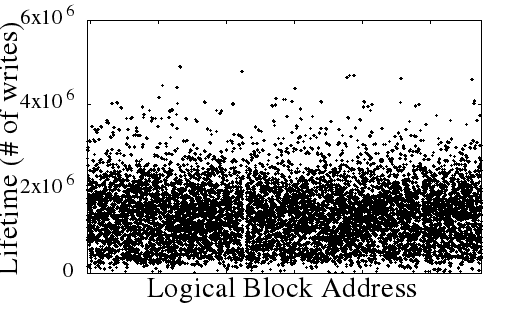
\includegraphics[width=0.19\textwidth]{figure/pc_3}}
	\hspace{2pt}
\subfloat[compaction: L2]{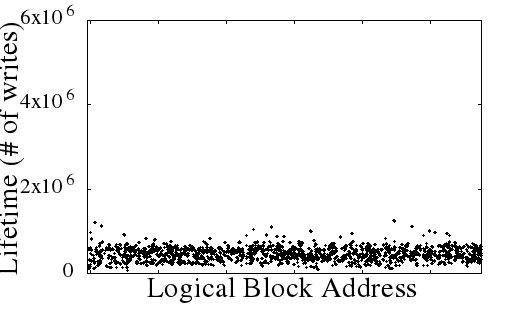
\includegraphics[width=0.19\textwidth]{figure/type_4}}  % data from 4/03040047
\hfill
\vspace{-1pt}
\subfloat[compaction: L3]{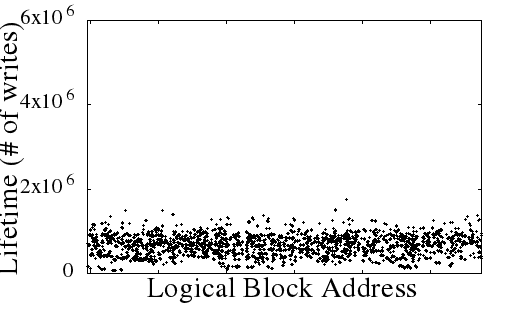
\includegraphics[width=0.19\textwidth]{figure/type_5}}
	\hspace{2pt}
\subfloat[compaction: L4]{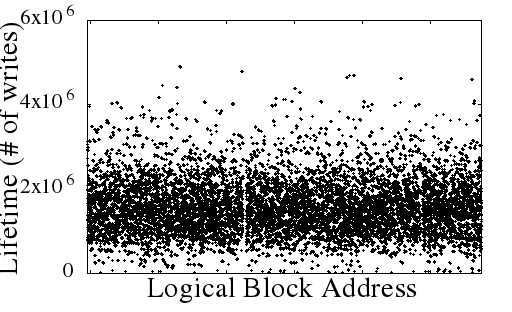
\includegraphics[width=0.19\textwidth]{figure/type_6}}
%\vspace{-10pt}
%\caption{The lifetime distribution of the compaction activity.} 
\caption{Lifetime distributions of the compaction activity at different levels.} %shane part
\label{fig:compaction}
%\vspace{-20pt}
\end{figure}

\subsection{Low resource requirement of internal streams}

In Section 2.2.1, we describe various resource overheads that limit the number of external streams.
In the case of an internal stream used for internal data migration of SSD, 
it has a relatively small resource overhead due to its distinguishing characteristics from the external stream.

Unlike external streams, which are handled directly by host requests,
since the internal stream can be processed as a background operation, 
performance degradation may not occur even if the data structure is located in a relatively slow memory.
However, the saturation condition, which requires GC to be continuously executed during write processing, 
may cause performance degradation due to relatively slow memory usage.

With regard to power resources, buffering can be used for flash parallelism even during data migration, but there is a big difference in that no power resource is required to guarantee data integrity.
In the case of buffering data for host write, if data is not stored in flash when power off, data is lost. 
However, in the case of buffering data during data migration, since the original data always exists in the source block of migration, there is no problem in ensuring data integrity without special handling or power resource requirement.

The increase of the active point for data migration has the problem that WAF might be increased by reducing the overprovision area. 
However, in most workloads, the benefit of using WAF reduction with multiple internal streams in data migration has the advantage of offsetting the increase in WAF due to overprovision area reduction and lowering the overall WAF.

\subsection{Internal Streams: Separating long-lived data during GC}
Since it is difficult to separate data with different lifetimes within the same PC 
(as in the compaction-activity PC), we devised a two-phase method that decides SSD 
streams in two levels: the main stream ID in a host level and the internal stream ID in an SSD level.
Conceptually, long-lived data in the main stream are moved to its internal stream to 
separate from (future) short-lived data of the main stream.
Although moving data to the internal stream may increase WAF,
the overhead can be hidden if we restrict the internal stream move during GC only.
Since long-lived data (i.e., valid pages) in a victim block are moved to a free block during GC, 
they can be moved to the internal stream by changing the target block.
For instance, \textsf{\small PCStream} assigns the compaction-activity PC {\it pID} to a
main stream {\it sID} for the first phase.
To separate the long-lived data of {\it pID} (e.g., L4 data) 
from future short-lived data of {\it pID} (e.g., L1 data), 
valid pages of the {\it sID} are assigned to its internal stream for the second phase during GC.




\section{Design and Implementation of \textsf{PCStream}}
In this section, we describe in detail the proposed automatic stream management technique,
\textsf{\small PCStream}.  We first explain how we automatically extract PCs during
runtime and describe how multiple PCs are mapped to streams in an SSD.

Fig.~\ref{fig:architecture} shows an overall organization of \textsf{\small PCStream}.
\textit{The PC extractor module}, which is implemented in the Linux kernel as
part of a system call handler, 
computes a PC signature, which is used as a unique ID for each program context.  
We use the signature program counter~\cite{PC} as a PC signature 
by summing program counter values along the execution path to a write-related system function 
(e.g., {\tt write()}).  
With the PC signature, we can monitor the data lifetime of each write at the program context level. 
A PC signature value is stored
in an inode data structure of a file system (modified for \textsf{\small PCStream})
and is delivered to \textit{the lifetime analyzer module} which estimates
expected lifetimes of data belonging to a given PC in the block device level.
In order to efficiently detect the end of data lifetime in append-only
workloads, the lifetime analyzer also intercepts TRIM~\cite{TRIM} requests from a file system.  %shane part
Based on the lifetime information, \textit{the PC-to-stream
mapper module} clusters PCs with similar lifetimes and maps them together to
the same stream ID.  This mapping is required because 
the number of streams in an SSD is generally less than the number of PCs in host applications.

\subsection{Automatic PC computation}
As mentioned earlier, a PC is represented by a PC signature which is defined as
the sum of program counter values along the execution path of a function call that
finally reaches a write-related system function. A function call involves
pushing the next program counter, which is used as a return address, to the
stack followed by pushing a frame pointer value.  In general, by using frame
pointer values, we are able to back-track the stack frames of the process and
selectively get return addresses for generating a PC signature.  For example,
Fig.~\ref{fig:getpc}(a) shows the abstracted execution path for flushing data
in RocksDB and Fig.~\ref{fig:getpc}(b) illustrates how a PC signature is obtained
by back-tracking the stack.  
Since a frame pointer value in the stack holds the address of the previous
frame pointer, the PC extractor can easily obtain return addresses and
accumulate them to compute a PC signature. 
(The return addresses are pushed
before calling the \textsf{\small  write()}, \textsf{\small  BuildTable()} and \textsf{\small 
WriteLevel0Table()} functions.)

\begin{figure}[t]
	\centering
	%\vspace{-10pt}
	%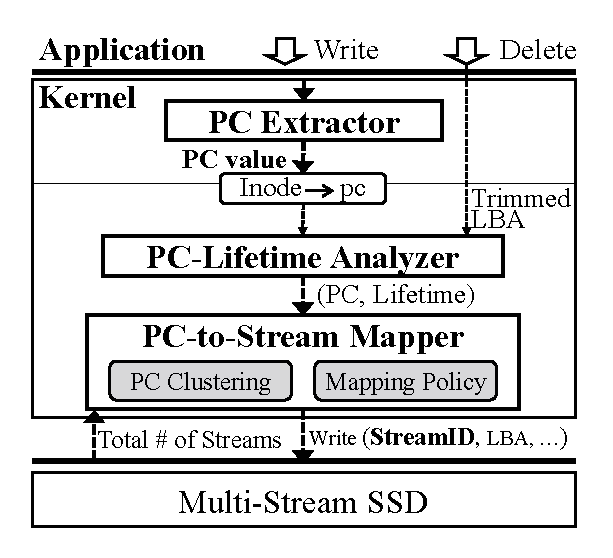
\includegraphics[width=0.6\linewidth]{figure/architecture4}
	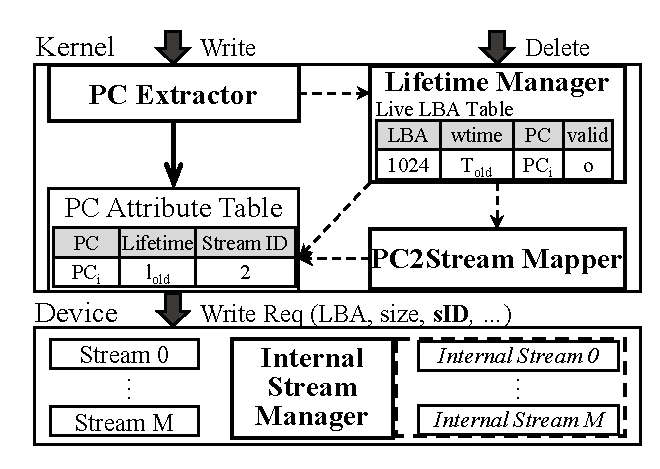
\includegraphics[width=0.6\linewidth]{figure/overview}
	%\vspace{-9pt}
	\caption{An overall architecture of \textsf{\small PCStream}.}
	\label{fig:architecture}
	%\vspace{-22pt}
\end{figure}


The frame pointer-based approach for computing PC signatures, however, is not
always possible because modern C/C++ compilers often do not use the frame
pointer for improving the efficiency of register allocation.
One example is a
{\tt -fomit-frame-pointer} option of GCC~\cite{GCC}. 
Although this option allows the frame pointer to be used as a general-purpose
register for high performance, it makes very difficult for us to back-track
return addresses along the call chains.  

\begin{figure}[b]
%	\vspace{-10pt}
	\centering
	%\vspace{-8pt}
	\subfloat[An abstracted execution path for flushing data.]{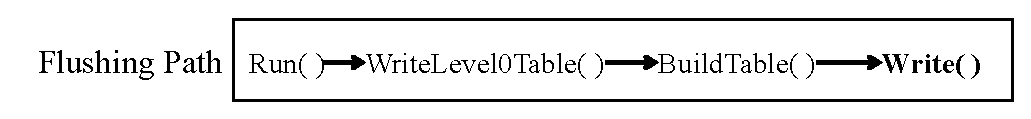
\includegraphics[width=0.4\textwidth]{figure/getpc_1}}  
	%\vspace{-14pt}
	\hfill
	\subfloat[with the frame pointer.]{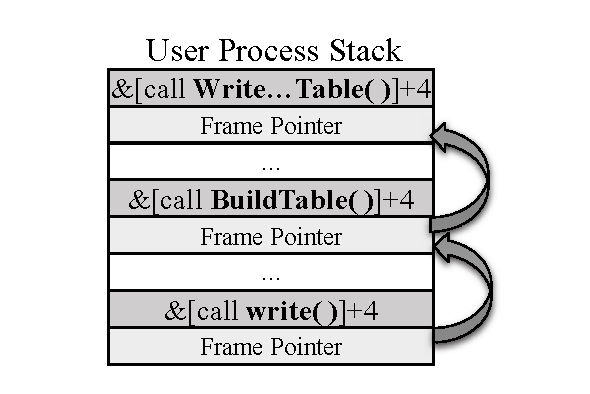
\includegraphics[width=0.22\textwidth]{figure/getpc_2}}
	\subfloat[without the frame pointer.]{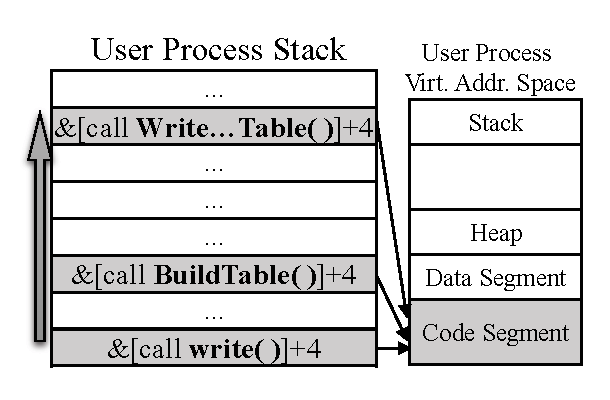
\includegraphics[width=0.22\textwidth]{figure/getpc_3}}
	%\vspace{-9pt}
	%\caption{An example execution path and its PC extraction methods.}
	\caption{An example execution path and its PC extraction.} %shane part
	\label{fig:getpc}
	%\vspace{-20pt}
\end{figure}

In \textsf{\small PCStream}, we employ a simple but effective workaround 
for backtracking the call stack when the frame pointer is not used.
When a write system call is made, we scan every word in the stack and check
if it belongs to the process's code segment.  If the scanned stack word holds a
value within the address range of the code segment, we assume that it is a
return address.  Since scanning the full stack takes too long, we stop the
stack scanning procedure when a sufficient number of return address candidates
are found.  In the current version, we stop when 5 return address candidates
are found.  Although quite ad-hoc, a restricted scan is effective in
distinguishing different PCs because two different PCs
cannot follow the same execution path to write system functions.  
(If they do, they are the same PC.) In our evaluation
with a 3.4 GHz CPU machine, the performance overhead of the restricted scan was
almost negligible, taking only 300-400 $n$sec per write system call.

\subsection{PC extraction for indirect writes}
{\color{blue}
앞서 언급한 방식은 write system call을 직접 호출하는 응용에 효과적이지만,
write system call을 직접 호출하지 않고 indirect write을 하는 응용에 대해서는 효과가 없다.
예를 들어, cassandra와 같이 JVM 기반의 응용은 write system call을 직접 호출하는 대신, Java가 제공하는 interface
를 사용하여 간접적으로 쓰기를 수행 한다.
이 경우, write system call 수준에서 PC를 추출하면, JVM 상에서 어떤 응용이 수행되고 있는지와는 관계없이 Java의
I/O를 담당하는 프로세스의 call stack만을 얻기 때문에 응용 프로그램의 I/O activity를 구분하려는 목적을 달성할 수 없다.
이러한 문제를 해결하기 위해서는 데이터가 만들어진 context를 정확히 파악할 수 있는 layer에서 PC가 계산 되어야 한다.
위의 예시에서는, system call layer 대신 Java interface를 통해 쓰기 요청을 전달 받을 때, PC extractor를 수행하면 의미있는
I/O activity를 구분할 수 있고 우리는 JDK를 수정하여 이러한 접근이 동작함을 확인하였다.
또 다른 indirect write case로, 프로그램 내부에 buffer를 유지하면서 이를 flushing하는 별도의 thread가 존재하는 경우가 있다.
이 역시 I/O activity를 구분할 수 있는 buffer에 데이터를 기록하는 시점에 구분되기 때문에, system call layer에서 PC를 추출하면 
의미 없는 flushing thread의 call stack만을 얻게 된다. 
그러나 이 case는 I/O activity가 구분되는 지점이 프로그램 내부의 function call로 이루어지기 때문에 프로그램이 이를 
알려주지 않는 이상 system 수준에서 이를 직접적으로 파악하기 어렵다. 
프로그램을 수정하지 않고 buffering의 I/O activity를 구분하는 문제는 이 논문에서 다루기에는
너무 복잡하기 때문에 future work으로 남긴다.
}

\subsection{PC lifetime management}
{\color{blue}Lifetime manager는 생성된 데이터의 수명을 계산하고 이를 PC 별로 구분하여 관리한다.
Lifetime Manager의 목적은 PC별 수명의 패턴을 파악하여 stream 할당의 기준을 만드는 것이다.
다양한 평가 결과, 우리는 동일한 I/O activity의 데이터라도 update 혹은 삭제 시기에 따라
개별적 데이터의 수명은 조금씩 달라지지만, 고유한 수명 패턴은 유지되는 것을 확인하였다.
따라서 lifetime manager는 수명의 정확한 값을 추구하기 보다는 수명의 대략적인 패턴을 파악하는 것을 목표로 한다.

데이터 lifetime은 쓰기 request가 issue된 때 부터 해당 주소가 다시 write되거나 
TRIM command에 의해 삭제될 때 까지로 정의된다.}
%The data lifetime of the append-only workload is defined 
%from when a write request is issued until the TRIM command~\cite{TRIM} is issued to 
%the corresponding address.
In order to measure the lifetime of data, the lifetime analyzer 
records the write time and PC value for each write request using its LBA.
Upon receiving the TRIM command or updating write request, the lifetime analyzer can compute the 
lifetime of the corresponding data using the recorded information.
{\color{blue} 
그러나 device 전체 LBA 공간에 대해 쓰여진 시간 정보를 유지하는 것은 메모리 부하가 크기 때문에,
우리는 1MB 크기의 chunk 단위로 나누어 관리하는 최적화 기법을 사용한다.
}
Note that, the
same PC may generate multiple data streams with different lifetimes.
We take the average lifetime as the PC's lifetime.

{\color{blue} Section 3에서 언급했듯이, PC는 user stack에 존재하는 
return address 즉, virtual address 기반으로 계산되므로
한 프로그램을 반복적으로 수행하면 동일한 PC들을 발견할 수 있다.
첫번째 수행 중 얻은 PC 별 lifetime 정보를 다음번 수행에서도 활용하기 위해 
이 정보를 유지하는 cache를 사용한다.
등장한 PC들과 그들의 lifetime 정보는 cache에 유지되고 추후 동일한 PC에 대해서는 
누적된 수명 정보를 활용할 수 있기 때문에 좀 더 정확한 수명 판단이 가능하다.
PC 값과 수명 값의 크기가 작기 때문에 몇십 KB의 메모리 만으로 충분히 많은 양의 데이터를 
유지할 수 있다. 따라서 본 논문에서는 PC cache replacement 정책에 대해서는 논의하지 않는다.
}

\subsection{Mapping PCs to SSD streams}

The last step in \textsf{\small PCStream} is to map
a group of PCs with similar lifetimes to an SSD stream.
This is because each SSD supports a limited number of stream IDs. For
example, SSDs used in \textsf{\small FStream}~\cite{FStream} and \textsf{\small AutoStream}~\cite{AutoStream}
support only 9 and 16 streams, respectively. 
{\color{blue} PC cluster는 비슷한 수준의 수명을 가진 PC들을 하나의 group으로 구분하기 위해 clustering algorithm을 사용한다.
본 연구에서는 overhead가 적고 많이 사용되는 k-means 알고리즘을 사용하였다.
SSD가 제공하는 stream의 개수와 동일한 group을 생성하여 각 PC group을 각 stream으로 할당한다.
}

%To properly group multiple PCs,
%the PC-to-stream mapper employs a simple 1-D clustering algorithm. 
%In order to cluster PCs with similar lifetimes, the mapper calculates the 
%lifetime difference between PCs.
%Then, PCs with the smallest lifetime difference are clustered into the same PC group. 
%The mapper repeats this clustering step until all the PCs are assigned to their PC groups.
{\color{blue} 추가로, SSD가 지원하는 stream의 개수가 변경되는 상황에서도 reclustering을 통해
대응이 가능하다.
For adapting to changing workloads, reclustering operations should be regularly performed. 
reclustering의 주기는 workload의 변화 패턴에 따라 결정될 수 있다.
새로운 PC가 계속적으로 생성되거나 한 PC의 수명 패턴이 자주 변화할 경우 reclustering의 주기를 
좀 더 짧게 설정하여 workload 변화를 반영한다.
}
%Since the
%number of PCs created by applications is not limited, the clustering algorithm
%must be efficient enough to quickly handle many PCs. 



\section{Experimental Results}

\textcolor{red}{(TODO: performance results are not included in section 6. we
should add some numbers such as runtime, throughput, cdf of latency, and SW
overhead)}

We have implemented \textsf{PCStream} on the Linux kernel 4.5 that runs on
Intel's i7-2600 CPUs with 8 cores and with 16~GB DRAM.  Samsung's PM963 480~GB
SSD with a multi-stream feature is used.  PM963 supports up to 9 streams; 8
user-configurable streams and one default stream. Write requests that do not
specify their stream IDs are assigned the default stream.  To support the
internal stream, we have modified the SSD firmware.  For detailed performance
analysis, an \texttt{nvme-cli} tool is modified to retrieve the information of
\textsf{PCStream}-enabled device internals, such as the WAF or
\textcolor{red}{the valid time of data in every blocks}.

%and its firmware has been modified to
%support the internal stream.

For an objective evaluation, we compared \textsf{\small PCStream} with three
existing schemes: \textsf{\small Baseline}, \textsf{\small
ManualStream}~\cite{MultiStream}, and \textsf{\small
AutoStream}~\cite{AutoStream}.  \textsf{\small Baseline} stands for a legacy
SSD that does not support multiple streams. \textsf{\small ManualStream}
represents multi-streamed SSDs with manual stream allocation.  \textsf{\small
AutoStream} is one that employs an LBA-based data separation technique which is
implemented at the device driver layer. 

We have carried out experiments with various benchmark programs, including
RocksDB~\cite{RocksDB}, Cassandra~\cite{Cassandra}, 
SQLite~\cite{SQLite}, and GCC~\cite{GCC}, each of
which generates distinct write patterns.  RocksDB and Cassandra have
append-only write patterns; SQLite has in-place update write patterns; GCC has
write-once patterns.  We also run the combinations of multiple programs
simultaneously for assessments under more realistic environments.  Yahoo! Cloud
Serving Benchmark (YCSB)~\cite{YCSB} with 120,000,000 keys runs on top of
RocksDB and Cassandra.  Both RocksDB and Cassandra are based on the LSM-tree
algorithm, so they have three major I/O activities (e.g.,
\textcolor{red}{logging, flush, and compaction}) as analyzed in Section 3.
%However, we identified about 5 PCs during runtime and we consider the extra
%PCs as management use.
TPC-C~\cite{TPCC} runs on SQLite with 20 warehouses.  Similarly, SQLite has two
major I/O activities (e.g., \textcolor{red}{logging and updating DB tables}). 
%2 kinds of data types in theory but we identified 4 PCs.
GCC compiles kernel source code 30 times. For the each run, 1/3 of source files
that are randomly chosen are modified and involved in the compilation.  GCC
creates many temporary files (e.g., \textcolor{red}{.s, .d, and .rc}) as well as long-lived
files (e.g., \textcolor{red}{.o}), thereby having more than 20 PCs.  To
generate mixed workloads, we run RocksDB and GCC scenarios together (denoted by
Mixed 1), and run SQLite and GCC scenarios at the same time (denoted by Mixed
2).
%Since GCC writes many kinds of temporary files as well as long-lived files,
%GCC has more than 20 PCs which makes clustering process effective for the GCC
%and mixed workloads.
To emulate an aged SSD, 90\% of the total SSD capacity was initially filled up
with user files before benchmarks run.


\subsection{WAF Comparison}

\begin{figure}[t]
	\centering
	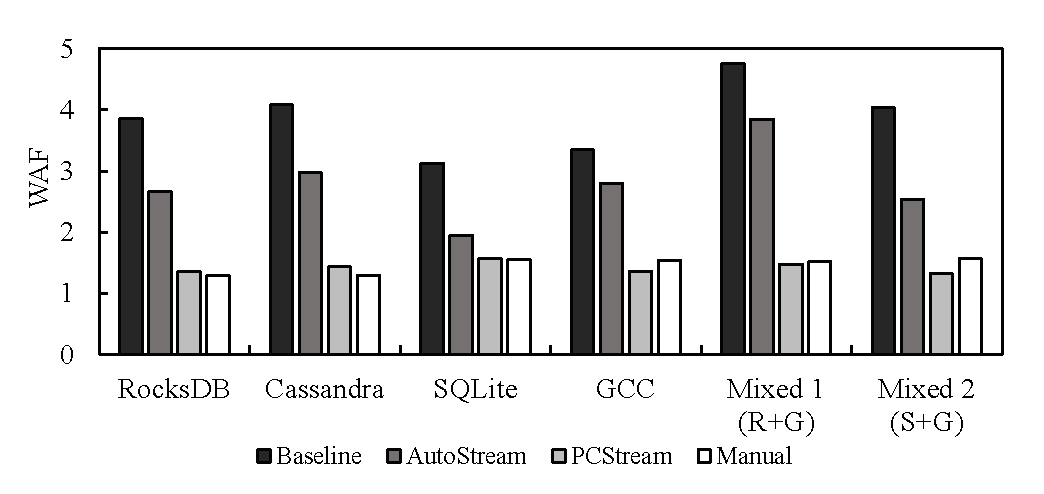
\includegraphics[width=0.9\linewidth]{figure/waf}
	\caption{The WAF comparison for various workloads.}
	\label{fig:waf}
	%\vspace{-36pt}
\end{figure}

We compared WAF of the existing techniques with \textsf{PCStream} for various
workloads, and the result is shown in Fig.~\ref{fig:waf}.  Overall,
\textsf{PCStream} was as efficient as \textsf{Manual}; Across all the
benchmarks, \textsf{PCStream} showed quite similar WAF values as
\textsf{Manual}. \textsf{PCStream} reduced WAF values by 63\% and 49\% over
\textsf{Baseline} and \textsf{AutoStream}, respectively, on average.  The
result shows that separating short-lived data (e.g., log or temp files) from
long-lived one (e.g., compaction or result files) using PC was quite effective.

As expected, \textsf{Baseline} showed the worst performance among all the
techniques.  We also observed that AutoStream was not able to achieve high WAF
reduction.  This was because the lack of relationship between hotness of data
and LBAs. Except for SQLite, all other benchmarks wrote data in an append-only
and/or a write-only manner. Since \textsf{PCStream} and \textsf{Manual} did not
depend upon LBAs for hot-cold separation, they performed well consistently,
regardless of write access patterns.


%Only SQLite had in-place update patterns for log files, 
%but the larger amount of data were written to database files 
%whose lifetimes are determined by the client
%which makes hard to predict their lifetime by the address.  In PCStream,
%however, long-lived data in database files are moved to internal streams during
%GC so that we can further reduce WAF.

One of the noticeable observations in Fig.~\ref{fig:waf} was that PCStream
performed even better than Manual for GCC, Mixed 1, and Mixed 2.  Those
benchmarks created many streams larger than ones supported by PM963.  In
\textsf{Manual}, application code was manually annotated at offline, so that
write I/Os from specific routines were assigned to designated SSD stream IDs.
Hence, it is impossible to know which applications run simultaneously, how many
streams would be created by them, and how to map those streams to SSD streams
in an optimal manner. Consequently, assigned stream IDs cannot be changed or
adjusted at run time adapting to the characteristics of programs running.
Unlike \textsf{Manual}, \textsf{PCStream} collected all PCs at run time,
clustered, and assigned them to SSD stream IDs, thereby outperforming
\textsf{Manual}.

%since the Manual scheme has static stream allocation.
%In Manual, once data types is mapped to the stream, the mapping is not changed 
%during runtime.
%For complex workloads which have large number of PCs such as mixed cases,
%it is difficult to expect data lifetimes in detail based on the data types.
%If the lifetime pattern is changed during runtime or the programmer choose
%second best stream mapping,
%Manual scheme lose the potential benefit in reducing WAf.
%However, the reclustering enables PCStream to adapt changing workload or find
%better stream mapping.
%The detailed analysis will be shown in the following subsections.

\begin{comment}
For example, both \textsf{\small PCStream} and \textsf{\small Manual} reduced WAF by 38\% over \textsf{\small Baseline} for the \texttt{UR} case. 
Compared with \textsf{\small AutoStream}, \textsf{\small PCStream} was more effective, reducing WAF more by 35\% on average.  
\textsf{\small PCStream} outperformed \textsf{\small AutoStream} by reducing WAF by 35\% on average.
Fig. 6 also indicates that the two-phase stream assignment technique is effective.  
\textsf{\small PCStream} outperformed \textsf{\small PCStream$^{*}$} by 12\% on average in the WAF reduction.
As shown in Fig. 6, \textsf{\small PCStream$^*$} reduced WAF by up to 30\% over \textsf{\small AutoStream}.  
\end{comment}

\subsection{Per-stream Lifetime Distribution Analysis}

\begin{figure}[t]
	\centering
	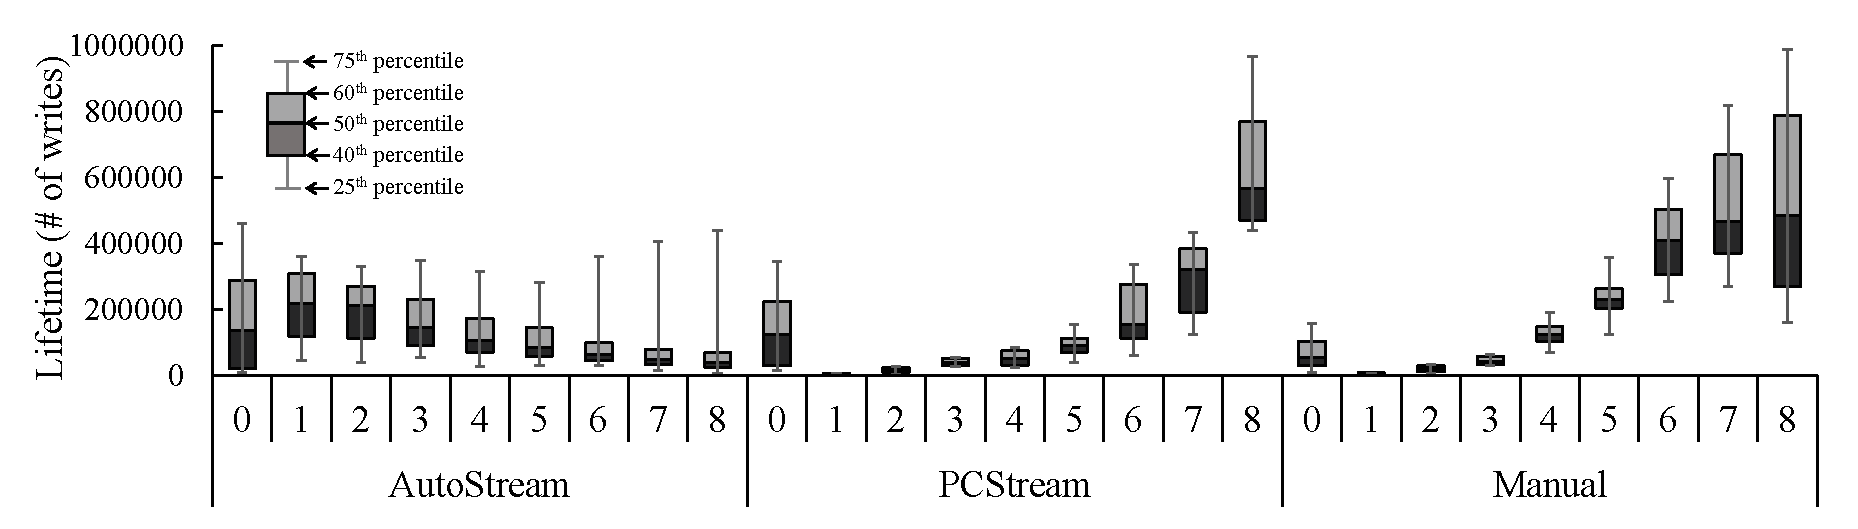
\includegraphics[width=1\linewidth]{figure/distribution}
	\caption{A Comparison of lifetime distributions of the smaller variance streams.}
	\label{fig:distribution}
	%\vspace{-36pt}
\end{figure}

To better understand the benefit of \textsf{\small PCStream} on WAF reduction,
we measured per-stream lifetime distributions for the \texttt{Mixed 1}
scenario.  Fig.~\ref{fig:distribution} shows a box plot of data lifetimes from
the 25th to the 75th percentile.  As shown in Fig.~\ref{fig:distribution},
streams in both \textsf{\small PCStream} and Manual are roughly categorized as
two groups, $G1$ = $\{$1, 2, 3, 4, 5$\}$ and $G2$ = $\{$6, 7, 8$\}$, where $G1$
includes streams with short lifetimes and small variances (i.e., streams 1, 2,
3, 4, and 5) and $G2$ includes streams with large lifetimes and large variances
(i.e., streams 6, 7, and 8). The stream 0 does not belong to any groups as it
is assigned to requests whose lifetimes are unknown.  Even though the variance
in the stream 0 is wider than that in Manual, PCStream showed similar
per-stream distributions as Manual. In particular, for the streams in $G2$,
PCStream exhibited smaller variance than Manual, which means that PCStream
separates cold data from hot data efficiently.

AutoStream was not able to achieve small variance of data lifetimes in
comparison with PCStream and Manual. At first, AutoStream assigns data to the
stream 0 and then increases the stream number according to their update
frequency. In Fig.~\ref{fig:distribution}, we found that short-lived data were
generally allocated to higher streams.  However, high variance observed across
all the streams indicates hot data are often mixed up with cold one.  This is
an expected result. In RocksDB and GCC workloads, there is no strong relation
between hotness of data and LBA.  Thus, long-lived data are often written to
LBAs where short-live data were previously written to, and it results in very
high lifetime variances for all the streams.

\subsection{Impact of the Internal Stream}

In order to understand the impact of the two-phase assignment, we compared each
technique with and without the internal stream.  The internal stream works
independently of a stream assignment method running at the host level, so it
can easily be combined with any host-level techniques.  Fig.~\ref{fig:internal}
shows a comparison of WAF values of Baseline, AutoStream, and PCStream under
the five workloads.  At a glance, we notice that all the techniques benefited
from using the internal stream.  However, its impact was not so high to offset
WAF costs caused by the improper stream assignment by the first-phase.  For
example, in Baseline, all the data from the host are first written to the same
default stream, regardless of their hotness.  Then, during SSD GC, cold data
that are left valid in the default stream are moved to the internal stream.
This helps us prevent cold data from being mixed up with future incoming data,
separating hot and cold data in two different segments. However, since the host
keeps writing the mixture of hot/cold data to the default stream, it is
impossible to avoid extra copy costs involved in the default stream.
AutoStream worked better than Baseline by assigning hot and cold data to
different streams, but owing to the inaccuracy of LBA-based hot-cold detection,
it performed worse than PCStream.

\begin{figure}[t]
	\centering
	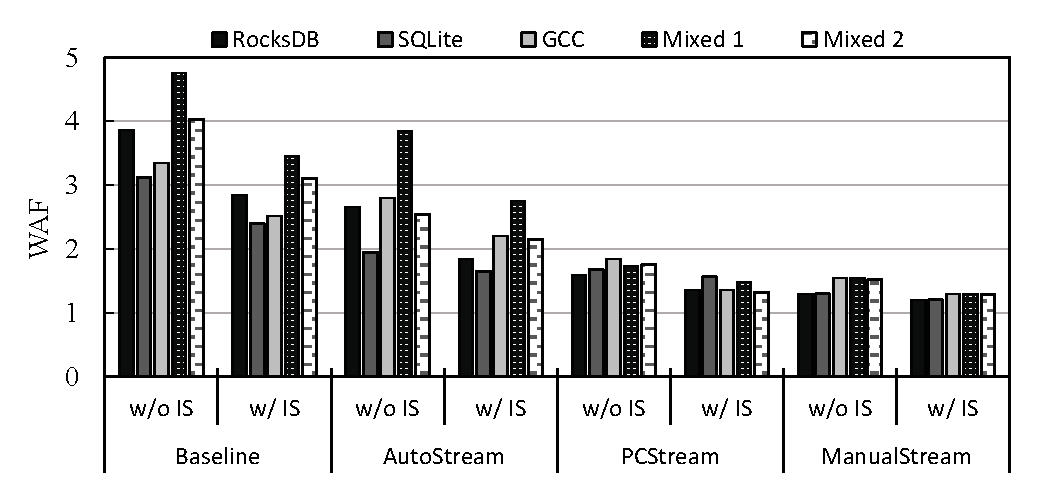
\includegraphics[width=0.9\linewidth]{figure/internal}
	\caption{Comparison of WAF w/ and w/o internal streams.}
	\label{fig:internal}
	%\vspace{-36pt}
\end{figure}


\subsection{Impact of the PC-stream table}

\begin{figure}[t]
	\centering
	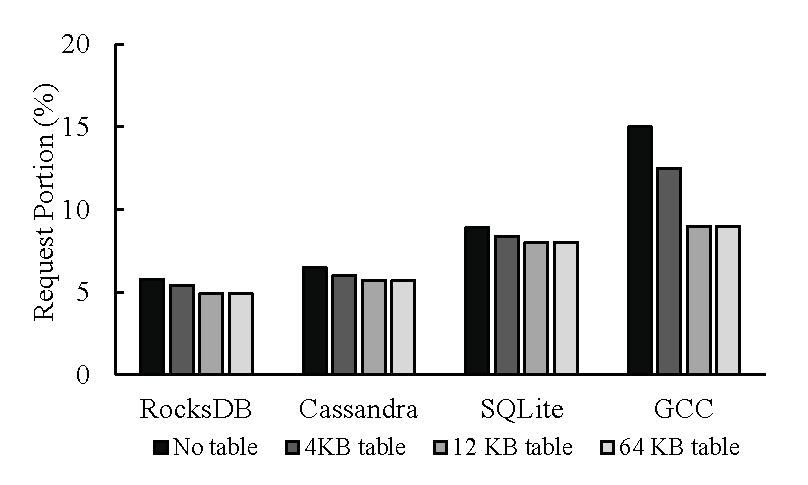
\includegraphics[width=0.7\linewidth]{figure/pctable}
	\caption{Request portion comparison of stream 0 with PC-stream table.}
	\label{fig:pctable}
	%\vspace{-36pt}
\end{figure}

As explained in Section 5, the PC-stream table provides us with a long-term
history of applications' I/O behaviors, and it even works for short-lived
applications that are frequently launched and terminated. To confirm its
benefits, we have modified \textsf{PCStream} so that it throws away the
contents of the PC-stream table at the end of each benchmark runs. For example,
in the kernel compilation scenario with GCC, the PC-stream table is
intentionally set empty after each run finishes, and thus the next run will
start without any prior knowledge about past PCs.

Fig.~\ref{fig:pctable} illustrates our experimental results, which shows how
many requests are sent to the stream 0. In \textsf{PCStream}, the stream 0 is
assigned to write requests whose lifetime behaviors are not estimated yet.
Therefore, the more write requests are assigned to the stream 0, the less the
history \textsf{PCStream} maintains. As shown in Fig.~\ref{fig:pctable}, in
RocksDB, Cassandra, and SQLite, the absence of the PC-stream table did not
affect the number of requests send to the stream 0. This is because those
programs ran continuously for a long time. Unlike them, GCC involves frequent
creations and termination of processes (e.g., \texttt{cc1}).
Hence, without the PC-stream table, about 16\% of requests were sent to the
stream 0. With the 4 KB-sized PC-stream table, it was reduced to 12\%
while with 12 KB-sized table, it was reduced to less than 10\%
and the result is saturated for tables larger than 12 KB.
We also
observed that with the PC-stream table, the WAF value was reduced from 1.96 to
1.54 for GCC.


\vspace{-10pt}
\section{Related Work}
\vspace{-5pt}

There have been many studies for multi-streamed SSDs ~\cite{MultiStream, Level,
vStream, FStream, AutoStream, PCStream}.  Kang {\it et al.} first proposed a
multi-streamed SSD that supported manual stream allocation for separating
different types of data~\cite{MultiStream}.  Yang {\it et al.} showed that a
multi-streamed SSD was effective for separating data of append-only
applications like RocksDB~\cite{Level}.  Yong {\it et al.} presented a virtual
stream management technique that resolved a limited number of streams.  While
above studies involve modifying the source code of target programs, the
stream allocation in PCStream is done automatically without any code
modification.

Rho {\it et al.} proposed a stream management technique, called FStream, at the
file system layer~\cite{FStream}. In FStream, metadata, journal
data, and user data that may have different lifetime characteristics were
allocated to separate streams.  Since FStream was implemented as part of a file
system, it was not able to directly detect application's I/O behaviors.
Also, it may be hard to be deployed in practice due to 
dependency with specific file-system implementations. PCStream is not
only able to detect application-specific behaviors, but also does not require
any modification of file systems.

Yang {\it et al.} presented the automatic stream management technique at the
block device layer. Similar to hot-cold separation employed in FTLs,
it decided the lifetime of data based on update frequencies of LBAs.
It didn't work well for applications ({\it e.g.}, RocksDB
and GCC) which have no a direct correlation between hotness of data
and LBAs.  PCStream detects the lifetime of data using PCs, so it
performs well even for append-only and write-once workloads.

Ha {\it et al.} proposed an idea of using PCs to separate hot data from cold
one in an FTL layer~\cite{PCHa}.  Kim {\it et al.} extended it for
multi-streamed SSDs~\cite{PCStream}.  Our work has improved the above
studies in a more complete fashion by showing 1) the important of the
internal stream guided by a host-level stream manager; 2) the effectiveness of
PCs for various workloads, including append-only, in-place update, and
write-once patterns; and 3) the unique and consistent nature of PCs which makes
it possible to capture long-term I/O behaviors of even short-lived
applications.



\vspace{-10pt}
\section{Conclusions}
\vspace{-5pt}

\begin{figure}[t]
	\centering
	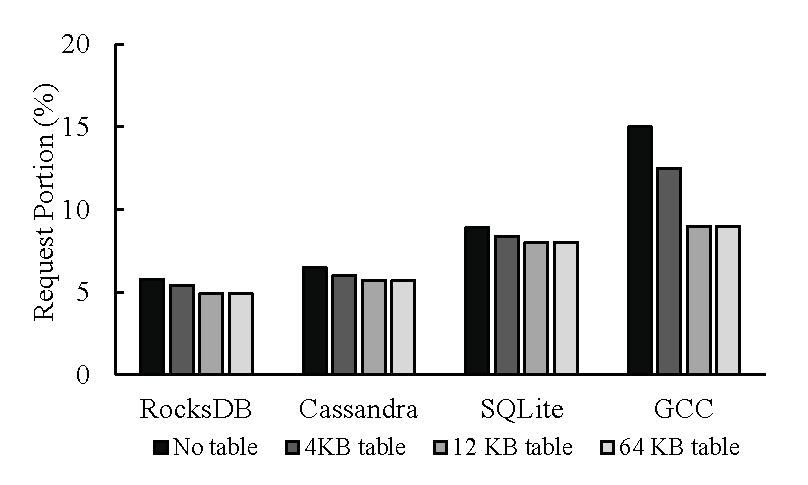
\includegraphics[width=0.87\linewidth]{figure/pctable}
	%\caption{The effect of the PC attribute table on the default stream allocation.}
	\caption{\note{The effect of the PC attribute table.}}
	\vspace{-5pt}
	\label{fig:pctable}
	\vspace{-10pt}
\end{figure}


We have presented a new stream management technique, \textsf{\small PCStream},
for multi-streamed SSDs.  Unlike existing techniques, \textsf{\small PCStream}
fully automates the process of mapping data to a stream based on PCs.  Based on
observations that most PCs are effective to distinguish lifetime
characteristics of written data, \textsf{\small PCStream} allocates each PC to
a different stream.  When a PC has a large variance in their lifetimes,
\textsf{\small PCStream} refines its stream allocation during GC and moves the
long-lived data of the current stream to the corresponding internal stream.
Our experimental results show that \textsf{\small PCStream} can improve the
IOPS by up to 56\% over the existing automatic technique while reducing WAF by
up to 69\%. 

The current version of \textsf{\small PCStream} can be extended in several
directions.  First, \textsf{\small PCStream} does not support applications that
rely on a write buffer ({\it e.g.,} MySQL). To address this, we plan to extend
\textsf{\small PCStream} interfaces so that developers can easily incorporate
\textsf{\small PCStream} into their write buffering modules with minimal
efforts.  Second, we have only considered write-related systems calls to
collect PCs, but many applications ({\it e.g.,} MonetDB~\cite{MonetDB}) heavily
access files with mmap-related functions ({\it e.g.}, \texttt{mmap()} and
\texttt{msync()}).  We plan to extend \textsf{\small PCStream} to work with
mmap-intensive applications. 




\begin{comment}
\section*{Acknowledgments}

This work was supported by the National Research Foundation of Korea (NRF) 
grant funded by the Korea government (Ministry
of Science and ICT) 
(NRF-2015M3C4A7065645 and NRF-2018R1A2B6006878).
The ICT at Seoul National University
provided research facilities for this study. 
Sungjin Lee was supported by
the NRF grant funded by the Korea government 
(Ministry of Science and ICT) 
(NRF-2017R1E1A1A01077410) and 
the DGIST R\&D Program of the Ministry of 
Science and ICT (18-EE-01).
(Corresponding Author: Jihong Kim)
\end{comment}

\newpage
\bibliographystyle{abbrv}
\bibliography{sigproc}
\begin{thebibliography}{00}

\bibitem{GCGreedy}
W. Bux, and I. Iliadis.
Performance of Greedy Garbage Collection in Flash-Based Solid-State Drives.
\textit{Performance Evaluation, vol. 67, no. 11, pp. 1172-1186}, 2010.

\bibitem{GCVictim}
C. Tsao, Y. Chang, and M. Yang.
Performance Enhancement of Garbage Collection for Flash Storage Devices: 
An Efficient Victim Block Selection Design.
In \textit{Proceedings of the 50th Annual Design Automation Conference (DAC'13)}, 2013.

\bibitem{GCTTFlash}
S. Yan, H. Li, M. Hao, M. Tong, S. Sundararaman, A. Chien, and H. Gunawi.
Tiny-tail Flash: Near-perfect Elimination of Garbage Collection Tail Latencies in NAND SSDs.
In \textit{Proceedings of the 15th USENIX Conference on File and Storage Technologies (FAST'17)}, 2017.

\bibitem{HotCold}
J. Hsieh, T. Kuo, and L. Chang.
Efficient Identification of Hot Data for Flash Memory Storage Systems.
\textit{ACM Transactions on Storage, vol. 2, no. 1, pp. 22-40}, 2006.

\bibitem{JiTGC}
S. Hahn, S. Lee, and J. Kim.
To Collect or Not to Collect: Just-in-Time Garbage Collection for High-Performance SSDs with Long Lifetimes
In \textit{Proceedings of the 52nd Design Automation Conference (DAC'15)}, 2015.

\bibitem{ShadowGC}
J. Cui, Y. Zhang, J. Huang, W. Wu, and J. Yang.
ShadowGC: Cooperative Garbage Collection with Multi-Level Buffer for Performance Improvement 
in NAND flash-based SSDs
In \textit{Proceedings of the 21th Design, Automation and Test in Europe Conference and Exhibition}, 2018.

\bibitem{T10}
SCSI Block Commnads-4 (SBC-4).
\url{http://www.t10.org/cgi-bin/ac.pl?t=f&f=sbc4r15.pdf}.

\bibitem{MultiStream}
J. Kang, J. Hyun, H. Maeng, and S. Cho. 
The Multi-streamed Solid-State Drive.
In \textit{Proceedings of the 6th Workshop on Hot Topics in Storage and File Systems (HotStorage'14)}, 2014.

\bibitem{Level}
F. Yang, D. Dou, S. Chen, M. Hou, J. Kang, and S. Cho.
Optimizing NoSQL DB on Flash: A Case Study of RocksDB.
In \textit{Proceedings of IEEE the 15th International Conference on Scalable Computing
and Communications (ScalCom'15)}. 2015.

\bibitem{FStream}
E. Rho, K. Joshi, S. Shin, N. Shetty, J. Hwang, S. Cho. and D. Lee. 
FStream: Managing Flash Streams in the File System.
In \textit{Proceedings of the 16th USENIX Conference on File and Storage Technologies (FAST'18)}, 2018.

\bibitem{vStream}
H. Yong, K. Jeong, J. Lee, J. Kim.
vStream: Virtual Stream Management for Multi-streamed SSDs.
In \textit{Proceedings of the 10th USENIX Workshop on Hot Topics in Storage
and File Systems (HotStorage'18)}, 2018.

\bibitem{AutoStream}
J. Yang, R. Pandurangan, C. Chio, and V. Balakrishnan.
AutoStream: Automatic Stream Management for Multi-streamed SSDs.
In \textit{Proceedings of the 10th ACM International Systems and Storage Conference (SYSTOR'17)}, 2017.

\bibitem{NVMe}
NVM Express Revision 1.3.
\url{http://nvmexpress.org/wp-content/uploads/NVM_Express_Revision_1.3.pdf}.

\bibitem{PCHa}
K. Ha, and J. Kim.
A Program Context-Aware Data Separation Technique for Reducing Garbage Collection Overhead in NAND Flash Memory.
In \textit{Proceedings of International Workshop on Storage Network Architecture 
and Parallel I/Os (SNAPI'11)}, 2011.

\bibitem{RocksDB}
Facebook. 
\url{https://github.com/facebook/rocksdb}.

\bibitem{Cassandra}
Apache Cassandra. 
\url{http://cassandra.apache.org}.

\bibitem{MySQL}
MySQL.
\url{https://www.mysql.com}.

\bibitem{PostgreSQL}
PostgreSQL.
\url{https://www.postgresql.org}.

\bibitem{OpenJDK}
OpenJDK.
\url{http://openjdk.java.net/}.

\bibitem{SQLite}
SQLite.
\url{https://www.sqlite.org/index.html}.

\bibitem{PC}
C. Gniady, A. Butt, and Y. Hu.
Program-Counter-Based Pattern Classification in Buffer Caching.
In \textit{Proceedings of the 6th Symposium on Operating Systems Design and Implementation (OSDI'04)}, 2004.

\bibitem{PC2}
F. Zhou, J. Behren, and E. Brewer.
Amp: Program Context Specific Buffer Caching.
In \textit{Proceedings of USENIX Annual Technical Conference (ATC'05)}, 2005.

\bibitem{kmeans}
J. Hartigan, and M. Wong.
Algorithm as 136: A k-means clustering algorithm.
\textit{Journal of the Royal Statistical Society. Series C (Applied Statistics),
vol. 28, no. 1, pp. 100-108}, 1979.

\bibitem{LSM}
P. ONeil, E. Cheng, D. Gawlick, and E. ONeil.
The Log-Structured Merge-Tree (LSM-Tree).
\textit{Acta Informatica, vol. 33, no. 4, pp. 351-385}, 1996.

\bibitem{TRIM}
J. Corbet.
Block Layer Discard Requests.
\url{https://lwn.net/Articles/293658/}.

\bibitem{GCC}
R. Stallman, and GCC Developer Community.
Using the GNU Compiler Collection for GCC version 7.3.0.
\url{https://gcc.gnu.org/onlinedocs/gcc-7.3.0/gcc.pdf}.


\bibitem{AMF}
S. Lee, M. Liu, S. Jun, S. Xu, J. Kim, and Arvind.
Application-Managed Flash.
In \textit{Proceedings of the 14th USENIX Conference on File and Storage
Technologies (FAST'16)}, 2016.

\bibitem{PCStream} 
T. Kim, S. Hahn, S. Lee, J. Hwang, J. Lee and J. Kim.
PCStream: Automatic Stream Allocation Using Program Contexts.
In \textit{Proceedings of the 10th USENIX Workshop on Hot Topics in Storage
and File Systems (HotStorage'18)}, 2018.



\end{thebibliography}


\theendnotes

\end{document}
